\chapter{Linker}

\section{Compiler Drivers}



\begin{lstlisting}[language=bash]
    linux> gcc -Og -o prog main.c sum.css

    cpp [other arguments] main.c /tmp/main.is
    as [other arguments] -o /tmp/main.o /tmp/main.s
    ld -o prog [system object files and args] /tmp/main.o /tmp/sum.o
    linux> ./prog
\end{lstlisting}

\begin{figure}[h!]
    \centering
    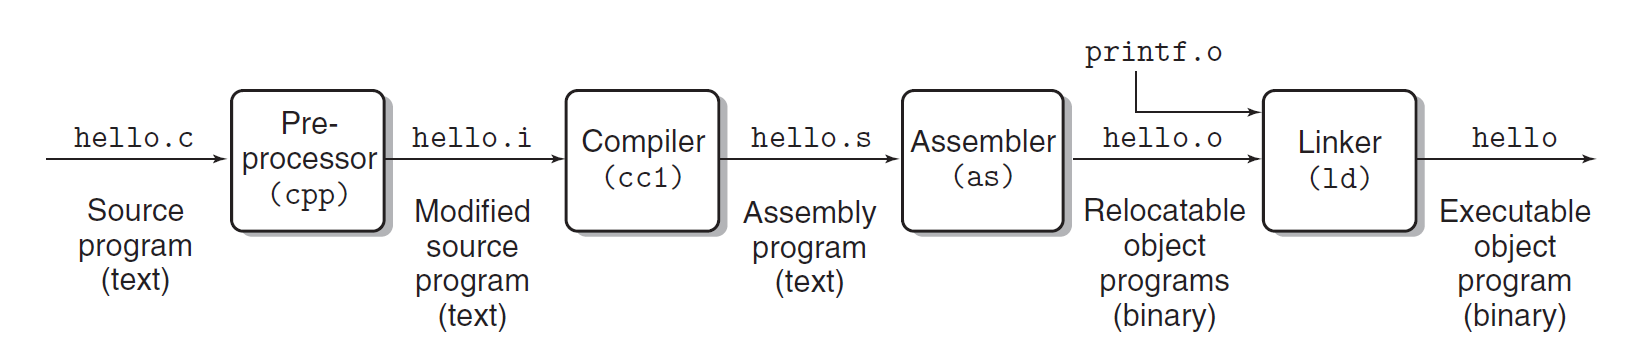
\includegraphics[scale=0.5]{pic/section7/pic1.png}
    \caption{Static linking. The linker combines relocatable    object files to form an executable object file prog}
\end{figure}



\section{Static Linking}

about symbol(7.5)
\begin{enumerate}
    \item symbol resolution(7.6)
    \item Relocation(7.7)
\end{enumerate}

\section{Object Files}

Object files are merely collections of blocks
of bytes. Some of these blocks contain program code, others contain program
data, and others contain data structures that guide the linker and loader. A linker
concatenates blocks together, decides on run-time locations for the concatenated
blocks, and modifies various locations within the code and data blocks. Linkers
have minimal understanding of the target machine. The compilers and assemblers
that generate the object files have already done most of the work.


\begin{itemize}
    \item Relocatable ob~(7.4) : compiler,assembler output
    \item Executable ob~(7.8,7.9) linker output
    \item shared ob~ (7.10)
\end{itemize}



\section{Relocatable Object Files}


\begin{figure}[h!]
    \centering
    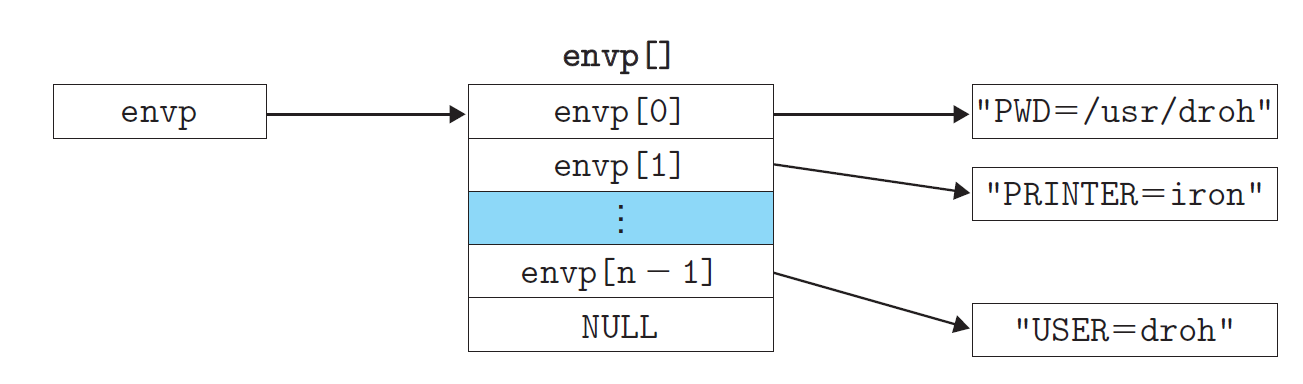
\includegraphics[scale=0.5]{pic/section7/pic2.png}
    \caption{Typical ELF relocatable object file.}
\end{figure}

\begin{itemize}
    \item \textbf{.text} The machine code of the compiled program.
    \item \textbf{.rodata} Read-only data such as the format strings in printf statements, and jump tables for switch statements.
    .data Initialized global and static C variables. Local C variables are maintained at run time on the stack and do not appear in either the .data or .bss sections.
    \item \textbf{.bss} Uninitialized global and static C variables, along with any global or static variables that are initialized to zero. This section occupies no actual space in the object file; it is merely a laceholder. Object file formats distinguish between initialized and uninitialized variables for space efficiency: uninitialized variables do not have to occupy any actual disk space in the object file. At run time, these variables are allocated in memory with an initial value of zero.
    \item \textbf{.symtab} A symbol table with information about functions and global variables
    that are defined and referenced in the program. Some programmers mistakenly believe that a program must be compiled with the -g option to
    get symbol table information. In fact, every relocatable object file has
    a symbol table in .symtab (unless the programmer has specifically removed it with the strip command). However, unlike the symbol table
    inside a compiler, the .symtab symbol table does not contain entries for
    local variables.
    \item \textbf{.rel.text} A list of locations in the .text section that will need to be modified
    when the linker combines this object file with others. In general, any
    instruction that calls an external function or references a global variable will need to be modified. On the other hand, instructions that call local functions do not need to be modified. Note that relocation information is not needed in executable object files, and is usually omitted unless the user explicitly instructs the linker to include it.
    \item \textbf{.rel.data} Relocation information for any global variables that are referenced or defined by the module. In general, any initialized global variable whose initial value is the address of a global variable or externally defined function will need to be modified.
    \item \textbf{.debug} A debugging symbol table with entries for local variables and typedefs defined in the program, global variables defined and referenced in the program, and the original C source file. It is only present if the compiler driver is invoked with the -g option.
    \item \textbf{.line} A mapping between line numbers in the original C source program and machine code instructions in the .text section. It is only present if the compiler driver is invoked with the -g option.
    \item \textbf{.strtab} A string table for the symbol tables in the .symtab and .debug sections and for the section names in the section headers. A string table is a sequence of null-terminated character strings.
\end{itemize}

\section{Symbols and Symbol Tables}

\begin{itemize}
    \item Global symbols that are defined by module m and that can be referenced by other modules :nonstatic C functions and global variables
    \item Global symbols that are referenced by module m but defined by some other module : nonstatic C functions and global variables that are defined in other modules.
    \item Local symbols that are defined and referenced exclusively by module m : nonstatic C functions and global variables that are defined in other modules.
\end{itemize}

\section{Symbol Resolution}

\subsection{How Linkers Resolve Duplicate Symbol Name}

\begin{itemize}
    \item strong symbol : 초기화된 전역변수
    \item weak symbol : 초기화x 전역변수
\end{itemize}

Rule
\begin{enumerate}
    \item Multiple strong symbols with the same name are not allowed.
    \item Given a strong symbol and multiple weak symbols with the same name, choose the strong symbol.
    \item Given multiple weak symbols with the same name, choose any of the weak symbols.
\end{enumerate}

\subsection{Linking with Static Libraries}

라이브러리 생성

\begin{lstlisting}[language=bash]
linux> gcc -c addvec.c multvec.c
linux> ar rcs libvector.a addvec.o multvec.o
\end{lstlisting}

라이브러리 링킹

\begin{lstlisting}[language=bash]
    
linux> gcc -c main2.c
linux> gcc -static -o prog2c main2.o ./libvector.a

linux> gcc -c main2.c
linux> gcc -static -o prog2c main2.o -L. -lvector

\end{lstlisting}

\begin{figure}[h!]
    \centering
    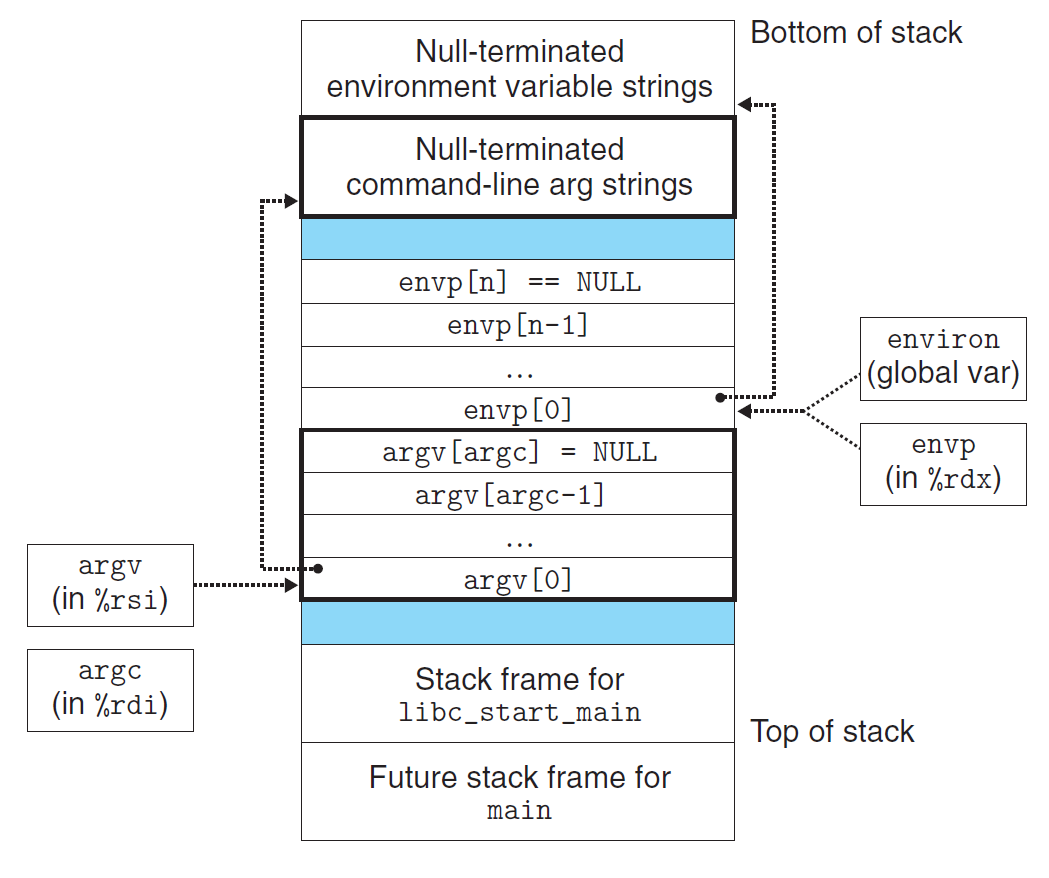
\includegraphics[scale=0.5]{pic/section7/pic3.png}
    \caption{Linking with static libraries.}
\end{figure}




\section{Relocation}

\begin{enumerate}
    \item Relocating sections and symbol definitionss :  여러개의 .data section 합친다. 이후 인스트럭션과 전역변수들이 런타임 메모리 주소를 가진다.
    \item Relocating symbol references within sections. :모든 심볼 참조를 수정한다. 이후  
    모든 심볼들이 런타임 메모리 주소를 가진다.
\end{enumerate}

\subsection{Relocation Entries}
위치를 모르는 심볼을 어떻게 처리할지에대해 어셈블러가만듬
.rel.data section에 존재

재배치방식
\begin{itemize}
    \item R\_X86\_64\_PC32 : 상대주소
    \item R\_X86\_64\_32. : 절대주소
\end{itemize}

\subsection{Relocating Symbol References}


\section{Executable Object Files}


\begin{figure}[h!]
    \centering
    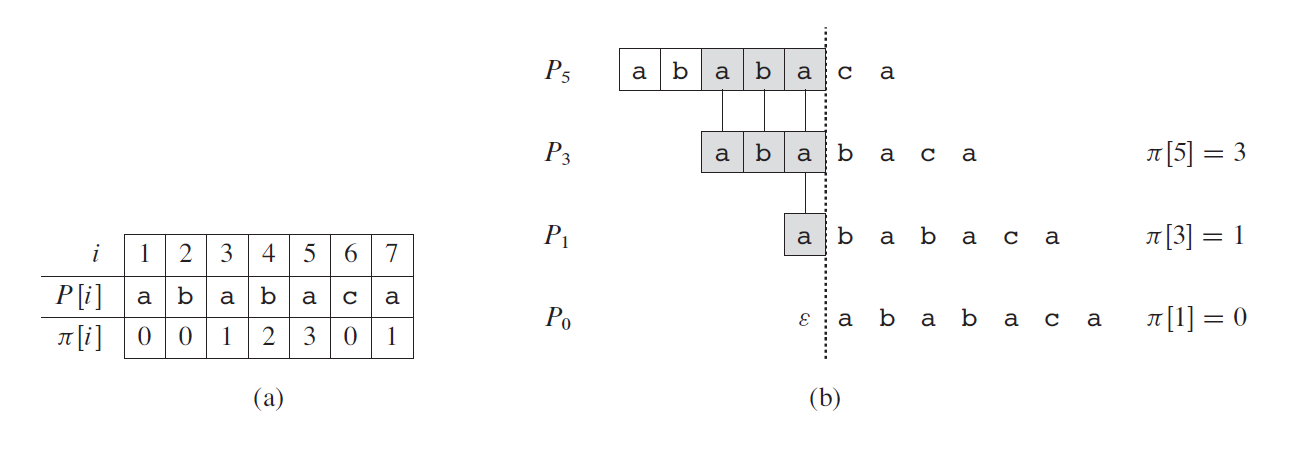
\includegraphics[scale=0.4]{pic/section7/pic4.png}
    \caption{Typical ELF executable object file.}
\end{figure}

\section{Loading Executable Object Files}

\begin{figure}[h!]
    \centering
    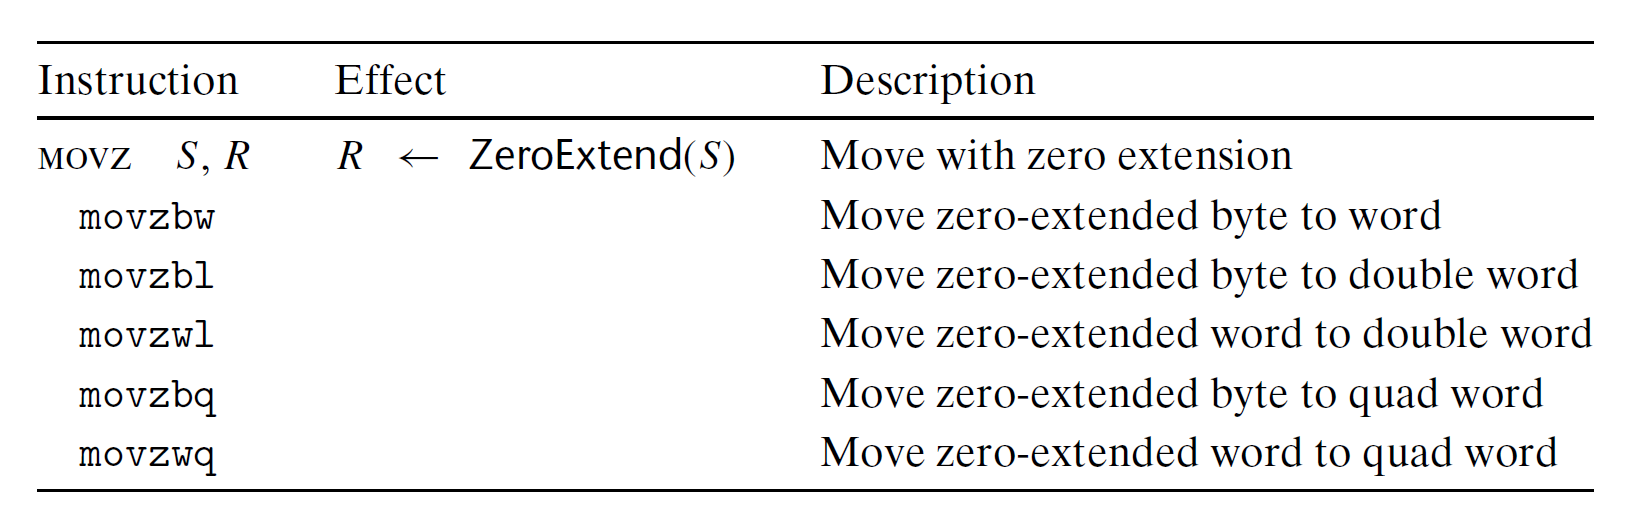
\includegraphics[scale=0.5]{pic/section7/pic5.png}
    \caption{\textbf{Linux x86-64 run-time memory image.} 
    Gaps due to segment alignment requirements and addressspace layout randomization (ASLR) are not shown. Not to scale}
\end{figure}

loading : 실행가능한 목적파일 내의 코드와 데이터를 메모리로 복사하고 첫번째 인스트럭션(엔트리 포인트)으로 점프해서실행하는 과정

\section{Dynamic Linking with Shared Libraries}

\begin{lstlisting}[language=bash]
linux> gcc -shared -fpic -o libvector.so addvec.c multvec.c
\end{lstlisting}

\begin{lstlisting}[language=bash]
    linux> gcc -o prog2l main2.c ./libvector.so
\end{lstlisting}

\begin{figure}[h!]
    \centering
    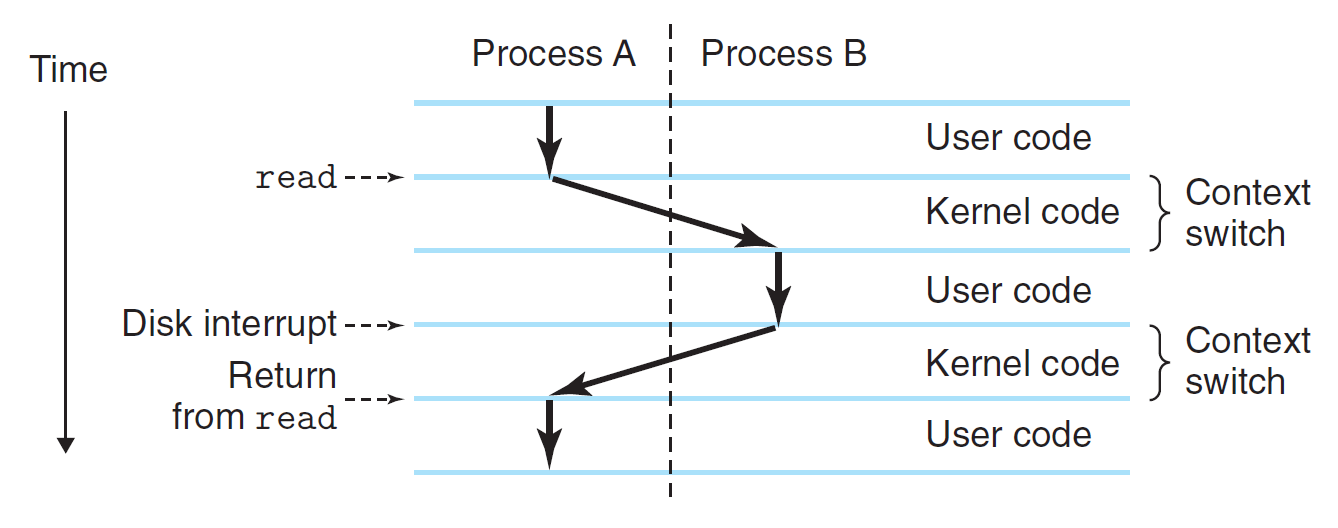
\includegraphics[scale=0.5]{pic/section7/pic6.png}
    \caption{Dynamic linking with shared libraries.}
\end{figure}



\section{Loading and Linking Shared Libraries from Applications}

\section{Position-Independent Code (PIC)}


\section{Library Interpositioning}
